%Version 3 December 2023
% See section 11 of the User Manual for version history
%
%%%%%%%%%%%%%%%%%%%%%%%%%%%%%%%%%%%%%%%%%%%%%%%%%%%%%%%%%%%%%%%%%%%%%%
%%                                                                 %%
%% Please do not use \input{...} to include other tex files.       %%
%% Submit your LaTeX manuscript as one .tex document.              %%
%%                                                                 %%
%% All additional figures and files should be attached             %%
%% separately and not embedded in the \TeX\ document itself.       %%
%%                                                                 %%
%%%%%%%%%%%%%%%%%%%%%%%%%%%%%%%%%%%%%%%%%%%%%%%%%%%%%%%%%%%%%%%%%%%%%

%%\documentclass[referee,sn-basic]{sn-jnl}% referee option is meant for double line spacing

%%=======================================================%%
%% to print line numbers in the margin use lineno option %%
%%=======================================================%%

%%\documentclass[lineno,sn-basic]{sn-jnl}% Basic Springer Nature Reference Style/Chemistry Reference Style

%%======================================================%%
%% to compile with pdflatex/xelatex use pdflatex option %%
%%======================================================%%

%%\documentclass[pdflatex,sn-basic]{sn-jnl}% Basic Springer Nature Reference Style/Chemistry Reference Style


%%Note: the following reference styles support Namedate and Numbered referencing. By default the style follows the most common style. To switch between the options you can add or remove “Numbered” in the optional parenthesis. 
%%The option is available for: sn-basic.bst, sn-vancouver.bst, sn-chicago.bst%  
 
%%\documentclass[pdflatex,sn-nature]{sn-jnl}% Style for submissions to Nature Portfolio journals
%%\documentclass[pdflatex,sn-basic]{sn-jnl}% Basic Springer Nature Reference Style/Chemistry Reference Style
\documentclass[pdflatex,sn-mathphys-num]{sn-jnl}% Math and Physical Sciences Numbered Reference Style 
%%\documentclass[pdflatex,sn-mathphys-ay]{sn-jnl}% Math and Physical Sciences Author Year Reference Style
%%\documentclass[pdflatex,sn-aps]{sn-jnl}% American Physical Society (APS) Reference Style
%%\documentclass[pdflatex,sn-vancouver,Numbered]{sn-jnl}% Vancouver Reference Style
%%\documentclass[pdflatex,sn-apa]{sn-jnl}% APA Reference Style 
%%\documentclass[pdflatex,sn-chicago]{sn-jnl}% Chicago-based Humanities Reference Style

%%%% Standard Packages
%%<additional latex packages if required can be included here>

\usepackage{graphicx}%
\usepackage{multirow}%
\usepackage{amsmath,amssymb,amsfonts}%
\usepackage{amsthm}%
\usepackage{mathrsfs}%
\usepackage[title]{appendix}%
\usepackage{xcolor}%
\usepackage{color, colortbl}
\usepackage{textcomp}%
\usepackage{manyfoot}%
\usepackage{booktabs}%
\usepackage{algorithm}%
\usepackage{algorithmicx}%
\usepackage{algpseudocode}%
\usepackage{listings}%
\usepackage{comment}
%%%%
\usepackage{tikz}
\usetikzlibrary{shapes.geometric, arrows, positioning}

% TikZ styles
\tikzstyle{startstop} = [rectangle, rounded corners, minimum width=3cm, minimum height=1cm,text centered, draw=black, fill=red!30]
\tikzstyle{process} = [rectangle, minimum width=3cm, minimum height=1cm, text centered, draw=black, fill=blue!30]
\tikzstyle{decision} = [diamond, minimum width=3cm, minimum height=1cm, text centered, draw=black, fill=green!30]
\tikzstyle{arrow} = [thick,->,>=stealth]
%%%%

%% as per the requirement new theorem styles can be included as shown below
\theoremstyle{thmstyleone}%
\newtheorem{theorem}{Theorem}%  meant for continuous numbers
%%\newtheorem{theorem}{Theorem}[section]% meant for sectionwise numbers
%% optional argument [theorem] produces theorem numbering sequence instead of independent numbers for Proposition
\newtheorem{proposition}[theorem]{Proposition}% 
%%\newtheorem{proposition}{Proposition}% to get separate numbers for theorem and proposition etc.

\theoremstyle{thmstyletwo}%
\newtheorem{example}{Example}%
\newtheorem{remark}{Remark}%

\theoremstyle{thmstylethree}%
	\newtheorem{definition}{Definition}%

\raggedbottom
%%\unnumbered% uncomment this for unnumbered level heads

\begin{document}

\section{Methods}
\label{sec:methods}

\subsection{Notation}
We denote specific channel states using subscripts (e.g., \( i, j \)), while superscripts (e.g., "prior", "post", "obs") are used to indicate the type of probability distribution (e.g., prior, posterior, or observed). For instance, \( p_i^{\text{prior}} \) represents the prior probability of being in state \( i \), and \( p_i^{\text{post}} \) represents the posterior probability after an observation.

\subsection{Markov model of single-channel behavior}

Early studies of single-channel recordings revealed that ion channels exhibit stochastic opening and closing at irregular intervals, consistent with the thermal fluctuations that macromolecules experience. Given this stochastic behavior, it is natural to model channel kinetics using a Markov process with a finite set of states \( k \), where each state represents a subset of the channel protein’s conformational landscape. 

A Markov process does not specify the precise conformation of the channel at any given moment; instead, it yields the probability vector \( \boldsymbol{p} \), where each element \( p_i \) represents the likelihood of the channel being in state \( i \). The model assumes a constant transition rate, \( k_{ij} \), for jumps between states \( i \) and \( j \). The time evolution of the probability vector \( \boldsymbol{p}(t) \) is governed by the following first-order differential equation:

\begin{equation}
	\frac{d \boldsymbol{p}}{dt}(t) = \boldsymbol{p}(t) \cdot \boldsymbol{Q}(t),
	\label{eq:master_equation}
\end{equation}

where the off-diagonal elements of the matrix \( \boldsymbol{Q} \) are given by the transition rates \( k_{ij} \). The diagonal elements \( k_{ii} \) are defined to ensure probability conservation:

\begin{align}
	k_{ii} = -\sum_{j, j \neq i} k_{ij}.
	\label{eq:Q_diagonal_element}
\end{align}

This formulation ensures that the total probability remains normalized over time, with the transitions between states governed by the rates encoded in the matrix \( \boldsymbol{Q} \). The Markovian framework thus reduces the complex conformational dynamics of the channel into a tractable probabilistic model, allowing for detailed analysis of the channel gating kinetics.


The integration of Eq.~\ref{eq:master_equation} allows us to determine the time evolution of the probability vector \( \boldsymbol{p}(t) \). This integration yields:


\begin{align}
	\boldsymbol{p}(t) &= \boldsymbol{p}(0) \cdot \boldsymbol{P}(t)
	\label{eq:master_equation_solution}
\end{align}
\begin{align}
	\boldsymbol{P} (t) &= \exp(\boldsymbol{Q} \cdot t),
	\label{eq:Transition_Matrix_definition}
\end{align}


where \( \exp(\boldsymbol{Q} \cdot t) \) is the matrix exponential of \( \boldsymbol{Q} \) multiplied by time \( t \). 

In this context, the actual state of the Markov process remains unobservable; what can be directly measured is the current produced by the channel. Each state \( i \) of the channel generates a specific single-channel current, encoded in the current vector \( \boldsymbol{\gamma} \). The observable current at any given time is thus determined by the probability-weighted sum over all states, which can be expressed as:

\begin{equation}
	y^{\text{pred}}(t) = \boldsymbol{p}(t) \cdot \boldsymbol{\gamma}.
	\label{eq:single_channel_prediction}
\end{equation}

This relationship links the hidden Markov states to the measurable macroscopic current, allowing us to infer the channel kinetics from experimental recordings.


\begin{algorithm}
	\caption{Markov Model of Single-Channel Behavior}\label{algo:markov_model}
	\begin{algorithmic}[1]
		\Require Transition rate matrix \( \boldsymbol{Q} \) and initial state probability vector \( \boldsymbol{p}(0) \)
		\Ensure Time-evolved probability vector \( \boldsymbol{p}(t) \) and predicted current \( y^{\text{pred}}(t) \)
		\Statex
		\State \textbf{Initialize:} Set \( \boldsymbol{p}(0) \), define \( \boldsymbol{\gamma} \) (current vector)
		\State \textbf{Define Transition Rate Matrix:} 
		\ForAll{states \( i, j \)} 
		\If{\( i \neq j \)}
		\State \( Q_{ij} \gets k_{ij} \) \Comment{Transition rate from \( i \) to \( j \)}
		\EndIf
		\State \( Q_{ii} \gets -\sum_{j \neq i} Q_{ij} \) \Comment{Ensure probability conservation}
		\EndFor
		\State \textbf{Compute Transition Matrix:}
		\State \( \boldsymbol{P}(t) \gets \exp(\boldsymbol{Q} \cdot t) \) \Comment{Matrix exponential}
		\State \textbf{Integrate Master Equation:}
		\State \( \boldsymbol{p}(t) \gets \boldsymbol{p}(0) \cdot \boldsymbol{P}(t) \) \Comment{Time evolution of \( \boldsymbol{p}(t) \)}
		\State \textbf{Compute Predicted Current:}
		\State \( y^{\text{pred}}(t) \gets \boldsymbol{p}(t) \cdot \boldsymbol{\gamma} \)
		\State \textbf{Output:} \( \boldsymbol{p}(t) \), \( y^{\text{pred}}(t) \)
	\end{algorithmic}
\end{algorithm}


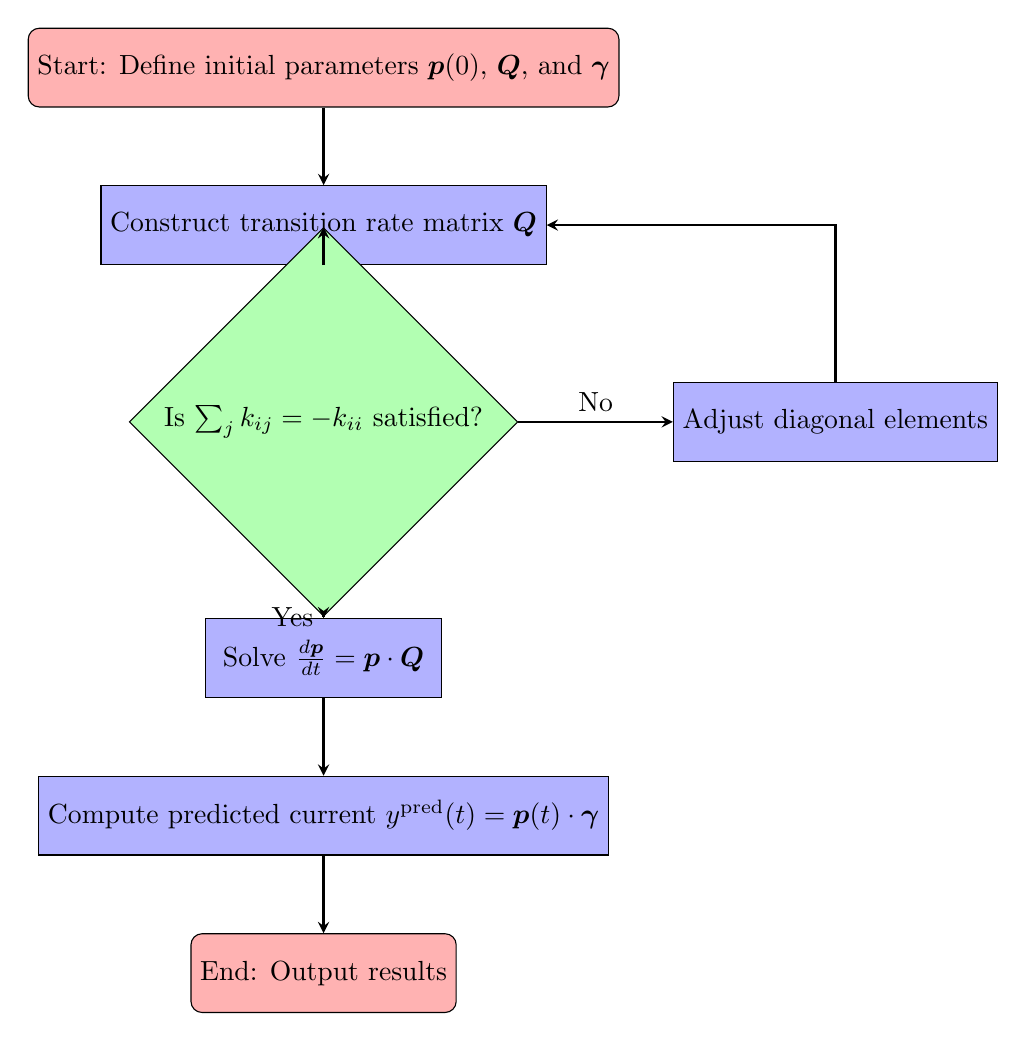
\begin{tikzpicture}[node distance=2cm]
	
	% Nodes
	\node (start) [startstop] {Start: Define initial parameters \( \boldsymbol{p}(0) \), \( \boldsymbol{Q} \), and \( \boldsymbol{\gamma} \)};
	\node (calculateQ) [process, below of=start] {Construct transition rate matrix \( \boldsymbol{Q} \)};
	\node (checkDiagonal) [decision, below of=calculateQ, yshift=-0.5cm] {Is \( \sum_j k_{ij} = -k_{ii} \) satisfied?};
	\node (fixQ) [process, right of=checkDiagonal, xshift=4.5cm] {Adjust diagonal elements};
	\node (solveODE) [process, below of=checkDiagonal, yshift=-1cm] {Solve \( \frac{d \boldsymbol{p}}{dt} = \boldsymbol{p} \cdot \boldsymbol{Q} \)};
	\node (current) [process, below of=solveODE] {Compute predicted current \( y^\text{pred}(t) = \boldsymbol{p}(t) \cdot \boldsymbol{\gamma} \)};
	\node (end) [startstop, below of=current] {End: Output results};
	
	% Arrows
	\draw [arrow] (start) -- (calculateQ);
	\draw [arrow] (calculateQ) -- (checkDiagonal);
	\draw [arrow] (checkDiagonal) -- node[anchor=south] {No} (fixQ);
	\draw [arrow] (fixQ) |- (calculateQ);
	\draw [arrow] (checkDiagonal) -- node[anchor=east] {Yes} (solveODE);
	\draw [arrow] (solveODE) -- (current);
	\draw [arrow] (current) -- (end);
	
\end{tikzpicture}

\subsection{MicroR, Bayesian model for instantaneous measurements of single-channel behavior}

The microscopic recursive term was coined for the exact description of an ensemble of channels, however the equations are the same that for single channels, so we extend the term to cover the classical bayesian analysis fo single channels. 
Consider the scenario where we perform a single "instantaneous" current measurement, denoted as \( y^{\text{obs}} \). Let the initial state probability distribution be given by \( \boldsymbol{p}^{\text{prior}} \). Suppose the instrumental noise associated with each measurement follows a normal distribution with variance \( \epsilon^2 \). Under these conditions, we can derive the likelihood of the measurement and update the posterior probability distribution accordingly.

Using the state current $\gamma_i$, the likelihood of observing the current \( y^{\text{obs}} \) is given by:

\begin{equation}
	\mathcal{L} = P(y^{\text{obs}}) = \sum_i \mathcal{N}(p_i \cdot \gamma_i, \epsilon^2),
	\label{eq:single_channel_likelihood}
\end{equation}

where \( \mathcal{N}(\mu, \sigma^2) \) denotes the normal distribution with mean \( \mu \) and variance \( \sigma^2 \).

The posterior probability distribution, \( \boldsymbol{p}^{\text{post}} \), is then updated using Bayes' rule:

\begin{equation}
	p^{\text{post}}_i = p_i \cdot \frac{\mathcal{N}(p_i \cdot \gamma_i, \epsilon^2)}{P(y^{\text{obs}})},
	\label{eq:single_channel_posterior}
\end{equation}

where \( p^{\text{post}}_i \) denotes the posterior probability of state \( i \) after observing the measurement.

Now, suppose a second measurement is taken after a time interval \( t \). The prior probability distribution at time \( t \), denoted \( \boldsymbol{p}^{\text{prior}}(t) \), is obtained by applying Eq.~\ref{eq:master_equation_solution}:

\begin{align}
	\boldsymbol{p}^{\text{prior}}(t) &= \boldsymbol{p}^{\text{post}}(0) \cdot \boldsymbol{P}(t)
	\label{eq:prior_update}
\end{align}

where \( \boldsymbol{Q} \) is the rate matrix governing the Markov process.

Since the probability of each observation \( {y}_n^{\text{obs}} \) is calculated conditionally on the previous observations \( {y}_1^{\text{obs}}, \dots, {y}_{n-1}^{\text{obs}} \), the cumulative log-likelihood of the entire measurement series can be obtained:

\begin{equation}
	\log \mathcal{L} = \sum_i \log (\mathcal{L}_i),
	\label{eq:total_loglikelihood}
\end{equation}

where \( \mathcal{L}_i \) corresponds to the likelihood of the \( i \)-th measurement.


\subsection{MicroIR, the Bayesian Model of Time-Averaged Single-Channel Measurements}

This new algorithm allows to analyze hidden markovian processes where the information we gain from them results from a time-weighed averaged response,as opposed as from an instantaneous observation. It is another solution for the missing events problem, but from a different perspective, one that does not intend to idealize the recording but to directly calculate the likelihood. This would allow to compare the evidence of alternative kinetic models, something that is not straightforward when an idealization step is included.  
We did not actually used this algorithm in this paper, it was necessary conceptual step to present MacroIR. We present it for single channels, but a similar argument can be extended for other single molecule systems, where time averaging is even more compelling (like molecular motors). 
We consider a scenario where, instead of instantaneous measurements, we observe the time-averaged current \( \overline{y_t}^{\text{obs}} \) over a specific interval \( t \). During this time interval, the channel state fluctuates continuously, with each specific trajectory representing a point in an infinite-dimensional space—an unwieldy realm for statistical analysis. However, from a Bayesian perspective, there is only one crucial piece of information: the prior probability distribution at the beginning of each interval. The state probabilities at all subsequent times within the interval can be computed using Eq.~\ref{eq:master_equation_solution}. 

On the other hand, there is only one piece of information that we gain from the interval: the observed average current. Ideally, we would like to obtain the posterior probability at the end of the interval so that it can be used as the prior for the next interval. To correctly compute this posterior distribution, we must account for both the starting and ending states.

Given the prior state probability distribution \( \boldsymbol{p}^{\text{prior}} \) at the start of the interval, we can calculate the joint state probability matrix \( \boldsymbol{\Pi} \), where the elements \( \Pi_{i \rightarrow j} \) represent the probability of starting in state \( i \) and ending in state \( j \):

\begin{equation}
	\Pi_{i \rightarrow j}^{\text{prior}} = p^{\text{prior}}_i \cdot P_{i \rightarrow j}
	\label{eq:joint_state_probability}
\end{equation}

Here, \( P_{i \rightarrow j} \) denotes the probability of transitioning from state \( i \) to state \( j \).

Alternatively, in matrix form:

\begin{equation}
	\boldsymbol{\Pi}^{\text{prior}} = \mathrm{diag}(\boldsymbol{p}^{\text{prior}}) \cdot \mathbf{P}
	\label{eq:joint_state_probability_matrix}
\end{equation}

The probability of an observed average current \( \overline{y}^{\text{obs}} \) result form Eq.~\ref{eq:single_channel_likelihood}:

\begin{equation}
	\mathcal{L}=P(\overline{y}^{\text{obs}}) = \sum_{i, j} \Pi_{i \rightarrow j}^{\text{prior}} \cdot \mathcal{N}\left(\overline{y}^{\text{obs}} - \Pi_{i \rightarrow j}^{\text{prior}} \cdot \overline{\Gamma}_{i \rightarrow j}, \epsilon^2 + \sigma^2_{\overline{\Gamma}_{i \rightarrow j}}\right)
	\label{eq:single_channel_integrated_likelihood}
\end{equation}

where \( \overline{\Gamma}_{i \rightarrow j} \) and \( \sigma^2_{\overline{\Gamma}_{i \rightarrow j}} \) represent the average current and its variance for trajectories starting in state \( i \) and ending in state \( j \), respectively.

The posterior distribution of the joint state probability matrix is updated using Bayes' theorem:

\begin{equation}
	\Pi_{i \rightarrow j}^{\text{post}} = \frac{\Pi_{i \rightarrow j}^{\text{prior}} \cdot \mathcal{N}\left(\overline{y}^{\text{obs}} - \Pi_{i \rightarrow j}^{\text{prior}} \cdot \overline{\Gamma}_{i \rightarrow j}, \epsilon^2 + \sigma^2_{\overline{\Gamma}_{i \rightarrow j}}\right)}{P(\overline{y}^{\text{obs}})}
	\label{eq:single_channel_integrated_posterior}
\end{equation}

The prior state probability distribution for the next interval is then obtained by marginalizing over the initial state \( i \):

\begin{equation}
	p_j^{\text{prior}}(t_{n+1}) = \sum_i \Pi_{i \rightarrow j}^{\text{post}}(t_n)
	\label{eq:single_channel_integrated_next_prior}
\end{equation}

Since the probability of each observation \( \overline{y}_n^{\text{obs}} \) is calculated conditionally on the previous observations \( \overline{y}_1^{\text{obs}}, \dots, \overline{y}_{n-1}^{\text{obs}} \), the cumulative log-likelihood of the entire measurement series can be updated using Eq. \ref{eq:total_loglikelihood}:

\begin{equation}
	\log \mathcal{L}(\overline{y}_1^{\text{obs}}, \dots, \overline{y}_{n+1}^{\text{obs}}) = \log \mathcal{L}(\overline{y}_1^{\text{obs}}, \dots, \overline{y}_n^{\text{obs}}) + \log P(\overline{y}_{n+1}^{\text{obs}})
	\label{eq:single_channel_integrated_total_likelihood}
\end{equation}

While the exact distribution of the mean current is not strictly normal, we approximate it as such, assuming that instrumental noise dominates over gating noise.

\subsubsection{Calculation of the Average Current Conditional on Starting and Ending States}

We calculate the average current \( \overline{\Gamma}_{i \rightarrow j} \) and its variance \( \sigma^2_{\overline{\Gamma}_{i \rightarrow j}} \) for transitions from state \( i \) to state \( j \) during a measurement interval \( t \).

The average current \( \overline{\Gamma}_{i \rightarrow j} \) is computed as the time-weighted average of the current in each state, weighted by the probability of being in that state during the interval:

\begin{equation}
	\overline{\Gamma}_{i \rightarrow j} = \frac{1}{t \cdot P_{i \rightarrow j}} \int_0^t \sum_k P_{i \rightarrow k}(\tau) \, \gamma_k \, P_{k \rightarrow j}(t - \tau) \, d\tau
	\label{eq:gamma_ij_integral}
\end{equation}

Here, \( P_{i \rightarrow j} \) is the probability of transitioning from state \( i \) to state \( j \) within time \( t \), \( P_{i \rightarrow k}(\tau) \) denotes the probability of transitioning from state \( i \) to state \( k \) at time \( \tau \), and \( \gamma_k \) is the current associated with state \( k \).

To efficiently evaluate this integral, we use a spectral form of the matrix exponential, yielding a closed-form expression:

\begin{equation}
	\overline{\Gamma}_{i \rightarrow j} = \frac{1}{P_{i \rightarrow j}} \sum_{k, n_1, n_2} V_{i n_1} \cdot V^{-1}_{n_1 k} \cdot \gamma_k \cdot V_{k n_2} \cdot V^{-1}_{n_2 j} \cdot E_2(\lambda_{n_1} \cdot t, \lambda_{n_2} \cdot t)
	\label{eq:gamma_ij_formula}
\end{equation}

where:
- \( \mathbf{V} \) and \( \mathbf{V}^{-1} \) are the matrices of eigenvectors of the rate matrix \( \mathbf{Q} \) and its inverse, respectively.
- \( \boldsymbol{\lambda} \) is the vector of eigenvalues of \( \mathbf{Q} \).
- The function \( E_2(x, y) \) is defined as:

\begin{equation}
	E_2(x, y) = 
	\begin{cases}
		\frac{\exp(x) - \exp(y)}{x - y}, & \text{if } x \neq y \\
		\exp(x), & \text{if } x = y
	\end{cases}
    \label{eq:E_2}
\end{equation}


\subsubsection{Calculation of the Variance of the Average Current Conditional on Starting and Ending States}

The variance of the average current, conditional on starting in state \(i\) and ending in state \(j\), is defined as the difference between the expected square of the average current and the square of the expected current:

\begin{equation}
	\sigma^2 \overline{\Gamma}_{i \rightarrow j}=\text{Var}(\overline{\Gamma}_{i \rightarrow j}) = E(\overline{\Gamma}_{i \rightarrow j}^2) - P_{i \rightarrow j} \cdot \left( E(\overline{\Gamma}_{i \rightarrow j}) \right)^2
    \label{eq:sigma_gamma_expression}
\end{equation}

where \( E(\overline{\Gamma}_{i \rightarrow j}^2) \) is the expected square of the average current, and \( E(\overline{\Gamma}_{i \rightarrow j}) \) is the expected average current.


To calculate the expected square of the average current, we consider the time-weighted average of the product of the currents at each pair of time points within the interval. This involves summing over all possible intermediate states \(k_1\) and \(k_2\) for the first and second currents, respectively. Specifically, we integrate over the full time interval, accounting for all combinations of transition probabilities at each time point:

\begin{equation}
	E(\overline{\Gamma}_{i \rightarrow j}^2) = \frac{1}{t^2 P_{i \rightarrow j}} \int_0^t \int_0^{t-\tau_1} \sum_{k_1, k_2} P_{i \rightarrow k_1}(\tau_1) \gamma_{k_1} P_{k_1 \rightarrow k_2}(\tau_2) \gamma_{k_2} P_{k_2 \rightarrow j}(t-\tau_1-\tau_2) d\tau_1 d\tau_2
    \label{eq:sqr_gamma_integral}
\end{equation}

Here, \(P_{i \rightarrow k_1}(\tau_1)\) and \(P_{k_1 \rightarrow k_2}(\tau_2)\) represent the transition probabilities between states over the respective time intervals \(\tau_1\) and \(\tau_2\), and \(\gamma_{k_1}\) and \(\gamma_{k_2}\) denote the currents in those states.


By utilizing the spectral decomposition of the transition rate matrix, we can obtain a closed-form expression for the expected square of the average current. This allows us to express the quantity in terms of matrix products and the eigenvalues of the transition rate matrix, as shown below:

\begin{equation}
	E(\overline{\Gamma}_{i \rightarrow j}^2) = \frac{1}{P_{i \rightarrow j}} \sum_{k_1, k_2, n_1, n_2, n_3} V_{i n_1} \cdot V^{-1}_{n_1 k_1} \cdot \gamma_{k_1} \cdot V_{k_1 n_2} \cdot V^{-1}_{n_2 k_2} \cdot \gamma_{k_2} \cdot V_{k_2 n_3} \cdot V^{-1}_{n_3 j} E_3(\lambda_{n_1} \cdot t, \lambda_{n_2} \cdot t, \lambda_{n_3} \cdot t)
    \label{eq:sqr_gamma_formula}
\end{equation}

Here, \(E_3\) is a function that acts on the eigenvalues of the transition rate matrix, and is defined as follows:

\begin{equation}
	E_3(x,y,z)= 
	\begin{cases}
		E_{111}(x,y,z) & x\neq y, y\neq z, z\neq x \\
		E_{12}(x,y) & x\neq y, x\neq z, y = z \\
		E_{12}(y,z) & y\neq z, y\neq x, z = x \\
		E_{12}(z,x) & z\neq x, z\neq y, x = y \\
		\frac{1}{2} \cdot \exp(x) & x=y=z
	\end{cases}
	\label{eq:E_3}
\end{equation}

The function \(E_{12}(x, y)\) is defined as:

\begin{equation}
	E_{12}(x,y) = E_{1,11}(x, y, y) + \frac{\exp(y)}{y - x} \cdot \left(\frac{y - x - 1}{y - x}\right)
	\label{eq:E_12}
\end{equation}

Finally, \(E_{1,11}(x, y, z)\) is given by:

\begin{equation}
	E_{1,11}(x, y, z) = \frac{\exp(x)}{(x - y) \cdot (x - z)}
	\label{eq:E_1_11}
\end{equation}

These expressions allow us to compute the expected square of the average current in a system where the transitions between states are governed by a Markov process with a known transition rate matrix.






\subsection{From Single-Channel Analysis to Ensemble Channel Analysis}

When the only information available about an ensemble of ion channels is the state probability vector—which specifies the likelihood of each individual channel being in a particular state—a multinomial distribution describes the probability of observing each possible distinct state count vector. However, once we gain additional information by measuring the total current produced by the ensemble, we can update the posterior distribution of the ensemble state. This updated distribution not only deviates from a multinomial form but also exhibits inverse correlations between states that generate the same current. Although individual channels remain independent, the information we obtain about the ensemble as a whole introduces correlations, reminiscent of quantum entanglement. Thus, we require a method to characterize the posterior probability distribution of the ensemble state that adequately captures these induced correlations.

A precise yet computationally intensive approach involves constructing a vector—referred to as the \textit{ensemble state vector}—that encompasses all possible combinations of state counts and applying Bayes' rule to each entry individually. This method, which I term the \textit{Microscopic Recursive Algorithm}, was detailed in a previous publication (Moffatt, 2007). However, this approach quickly becomes computationally prohibitive as the system size increases.

A more efficient alternative approximates the ensemble state distribution using a multivariate normal distribution of the state count vector. The covariance matrix serves as a first-order approximation to account for the observation-induced correlations between states. This constitutes the \textit{Macroscopic Approach}, significantly simplifying the representation of the ensemble's state distribution.

\subsection{MacroR, Bayesian Framework for Instantaneous Measurements of Channel Ensembles}

In the \textit{MacroR algorithm}, we treat measurements as instantaneous and focus solely on the ensemble's instantaneous state. This framework leverages both the mean probability vector and the covariance matrix of the probability state, capturing the ensemble's key statistical properties at any given moment. The same results can be obtained from a Kalman filter. 

After integrating the multivariate Gaussian, the likelihood of observing an instantaneous current \( y^{\text{obs}} \) can be obtained:

\begin{equation}
	\mathcal{L} = \mathcal{N} \left( y^{\text{obs}} - y^{\text{pred}}, \sigma^2_{y^{\text{pred}}} \right)
	\label{eq:macro_likelihood}
\end{equation}

where \( y^{\text{pred}} \), the prediction of the kinetic model for the subsequent observation, is given by:

\begin{equation}
	y^{\text{pred}} = N_{\text{ch}} \cdot \boldsymbol{\mu}^{\text{prior}} \cdot \boldsymbol{\gamma}
	\label{eq:macro_predicted_y}
\end{equation}

Here, \( \sigma^2_{y^{\text{pred}}} \), the variance of this prediction, which is related to what is usually called gating noise, is:

\begin{equation}
	\sigma^2_{y^{\text{pred}}} = \epsilon^2 + N_{\text{ch}} \cdot \boldsymbol{\gamma}^{\mathrm{T}} \cdot \boldsymbol{\Sigma}^{\text{prior}} \cdot \boldsymbol{\gamma}
	\label{eq:macro_sigma_pred}
\end{equation}

Similarly, we have a closed form for \( \boldsymbol{\mu}^{\text{post}} \), the mean state probability vector, which is the mean of the multivariate Gaussian representing the posterior probability state:

\begin{equation}
	\boldsymbol{\mu}^{\text{post}} = \boldsymbol{\mu}^{\text{prior}} + \frac{y^{\text{obs}} - y^{\text{pred}}}{\sigma^2_{y^{\text{pred}}}} \cdot \boldsymbol{\gamma}^{\mathrm{T}} \cdot \boldsymbol{\Sigma}^{\text{prior}}
	\label{eq:macro_mean_posterior}
\end{equation}

And for \( \boldsymbol{\Sigma}^{\text{post}} \), the covariance of the state probability vector, which represents the covariance of the same multivariate Gaussian:

\begin{equation}
	\boldsymbol{\Sigma}^{\text{post}} = \boldsymbol{\Sigma}^{\text{prior}} - \frac{N}{\sigma^2_{y^{\text{pred}}}} \cdot \boldsymbol{\Sigma}^{\text{prior}} \cdot \boldsymbol{\gamma} \cdot \boldsymbol{\gamma}^{\mathrm{T}} \cdot \boldsymbol{\Sigma}^{\text{prior}}
	\label{eq:macro_cov_posterior}
\end{equation}

Next, we calculate the prior probability at time \( t_{n+1} = t_n + \Delta t_n \) using conditional expectation:

\begin{equation}
	\boldsymbol{\mu}^{\text{prior}}(t_{n+1}) = \boldsymbol{\mu}^{\text{post}}(t_n) \cdot \mathbf{P}(\Delta t_n)
	\label{eq:macro_mean_next_prior}
\end{equation}

And its covariance:

\begin{equation}
	\boldsymbol{\Sigma}^{\text{prior}}(t_{n+1}) = \mathrm{diag}(\boldsymbol{\mu}^{\text{prior}}(t_{n+1})) + \mathbf{P}(\Delta t_n)^{\mathrm{T}} \cdot \left( \boldsymbol{\Sigma}^{\text{post}}(t_n) - \boldsymbol{\mu}^{\text{post}}(t_n) \right) \cdot \mathbf{P}(\Delta t_n)
	\label{eq:macro_mean_next_cov}
\end{equation}

This completes the recursion step of the Macroscopic Recursive algorithm.


\subsection{MacroIR: A Bayesian Framework for Interval-Averaged Analysis of Channel Ensembles}

We introduce MacroIR (Macroscopic Interval Recursive), a novel Bayesian framework designed for time-averaged Markovian processes over successive intervals. The algorithm is inspired by macropatch recordings, which provide high-fidelity kinetic data with low noise. This approach is versatile, extending to systems such as FRET measurements, molecular motor ensembles, and potentially diffusion analyses.

MacroIR applies the MacroR algorithm to the meta-state described in the MicroIR algorithm, which represents the initial and final states within an interval. Importantly, while the meta-state concept theoretically expands the state space from \( k \) to \( k^2 \), leading to a computational cost scaling from \( k^3 \) to \( k^6 \), algebraic simplifications restore the complexity to \( k^3 \). These simplifications eliminate the need for explicit meta-state calculations, enabling efficient updates of the likelihood and posterior distributions.

The meta-state represents the joint probabilities of starting in state \( i_0 \) and ending in state \( i_t \) over a time interval \( [0, t] \). The prior mean is given by:
\begin{equation}
	(\mu^{\text{prior}}_{0 \rightarrow t})_{(i_0 \rightarrow i_t)} = (\mu^{\text{prior}})_{i_0} \cdot P_{i_0 \rightarrow i_t}(t),
	\label{eq:meta_mean_prior}
\end{equation}
where \( P_{i_0 \rightarrow i_t}(t) \) is the transition probability.

Similarly, the prior covariance is:
\begin{multline}
	(\Sigma^{\text{prior}}_{0 \rightarrow t})_{(i_0 \rightarrow i_t)(j_0 \rightarrow j_t)} = 
	P_{i_0 \rightarrow i_t} \big[(\Sigma^{\text{prior}}_0)_{i_0, j_0} - \delta_{i_0, j_0} \cdot (\mu^{\text{prior}}_0)_{i_0} \big] \cdot P_{j_0 \rightarrow j_t} \\
	+ \delta_{i_0, j_0} \cdot \delta_{i_t, j_t} \cdot (\mu^{\text{prior}}_0)_{i_0} \cdot P_{i_0 \rightarrow i_t},
	\label{eq:meta_covariance_prior}
\end{multline}
where \( \delta_{i, j} \) is the Kronecker delta.

The predicted average current over the interval is:
\begin{equation}
	\overline{y}^{\text{pred}}_{0,t} = N_{\text{ch}} \cdot \mathbf{\mu}^{\text{prior}}_{0} \cdot \overline{\gamma}_{0},
	\label{eq:macro_interval_predicted_y}
\end{equation}
where \( \overline{\gamma}_{0} \) is the average current marginalized over end states:
\begin{equation}
	(\overline{\mathbf{\gamma}}_{0})_i = \sum_j (\overline{\Gamma})_{i \rightarrow j}.
\end{equation}

The variance of the predicted current accounts for intrinsic channel noise and state transitions:
\begin{equation}
	\sigma^2_{\overline{y}^{\text{pred}}_{0 \rightarrow t}} = \epsilon^2_{0 \rightarrow t} + N_{\text{ch}} \cdot \widetilde{\mathbf{\gamma}^{\mathrm{T}} \mathbf{\Sigma}\mathbf{\gamma}} + 
	N_{\text{ch}} \cdot \mathbf{\mu}^{\mathrm{prior}}_{0} \cdot {\sigma^2 \overline{\mathbf{\gamma}}}_{0}.
	\label{eq:macro_interval_sigma_pred}
\end{equation}
Here, the variance of the average current conditional on the start state, \( \overline{\mathbf{\gamma}}_{0} \), is obtained by marginalizing over the end state:
\begin{equation}
	(\sigma^2_{\overline{\mathbf{\gamma}}_{0}})_i = \sum_j (\sigma^2 \overline{\Gamma})_{i \rightarrow j}.
	\label{eq:sigma_gamma_i}
\end{equation}

The expression for \( \widetilde{\mathbf{\gamma}^{\mathrm{T}} \mathbf{\Sigma}\mathbf{\gamma}} \) is given by:
\begin{multline}
	\widetilde{\mathbf{\gamma}^{\mathrm{T}} \mathbf{\Sigma}\mathbf{\gamma}}=   \mathbf{\gamma}^{\mathrm{T}}_{0 \rightarrow t} \cdot \mathbf{\Sigma}^{\mathrm{prior}}_{0 \rightarrow t} \cdot \mathbf{\gamma}_{0 \rightarrow t} = \\
	\overline{\mathbf{\gamma}}_{0}^{\mathrm{T}} \cdot 
	\left( \mathbf{\Sigma}^{\mathrm{prior}}_{0} - \mathrm{diag}(\mathbf{\mu}^{\mathrm{prior}}_0) \right) \cdot 
	\overline{\mathbf{\gamma}}_{0 \rightarrow t} \\
	+ \mathbf{\mu}^{\mathrm{prior}}_0 \cdot \left( \overline{\mathbf{\Gamma}}_{0 \rightarrow t} \circ \overline{\mathbf{\Gamma}}_{0 \rightarrow t} \circ \mathbf{P} \right) \cdot \mathbf{1}.
	\label{eq:simplified_meta_state}
\end{multline}
where \( \circ \) denotes the element-wise (Hadamard) product and \( \mathbf{1} \) is a vector of ones.

Posterior updates are efficiently computed without explicitly involving the meta-state:
\begin{equation}
	\boldsymbol{\mu}^{\mathrm{prior}}_{t} = 
	\boldsymbol{1}_0 \cdot 
	\boldsymbol{\mu}^{\mathrm{post}}_{0 \rightarrow t} = \boldsymbol{\mu}^{\mathrm{prior}}_0 \cdot \boldsymbol{P} + 
	\frac{y^{\mathrm{obs}}_{0 \rightarrow t} - y^{\mathrm{pred}}_{0 \rightarrow t}}{{\sigma^2}_{\overline{y}^{\mathrm{pred}}_{0 \rightarrow t}}} 
	\cdot \widetilde{\boldsymbol{\gamma}^{\mathrm{T}} \boldsymbol{\Sigma}}.
	\label{eq:macro_interval_posterior_mean}
\end{equation}
where left-multiplication by \( \mathbf{1}_0 \) represents the marginalization over the start state, and
\begin{equation}
	\widetilde{\boldsymbol{\gamma}^{\mathrm{T}} \boldsymbol{\Sigma}} = \mathbf{1}_0 \cdot \mathbf{\gamma}^{\mathrm{T}}_{0 \rightarrow t} \cdot \mathbf{\Sigma}^{\mathrm{prior}}_{0 \rightarrow t} =
	\overline{\boldsymbol{\gamma}}_{0}^{\mathrm{T}} \cdot 
	\left( \boldsymbol{\Sigma}^{\mathrm{prior}}_{0} - \mathrm{diag}(\boldsymbol{\mu}^{\mathrm{prior}}_0) \right) \cdot \boldsymbol{P} 
	+ \boldsymbol{\mu}^{\mathrm{prior}}_0 \cdot \left( \overline{\boldsymbol{\Gamma}}_{0 \rightarrow t} \circ \boldsymbol{P} \right).
	\label{eq:interval_gamma_sigma}
\end{equation}

The prior covariance for the next interval is derived by marginalizing over initial states:
\begin{multline}
	\boldsymbol{\Sigma}^{\mathrm{prior}}_{t} = 
	\boldsymbol{P}^{\mathrm{T}} \cdot \left( \boldsymbol{\Sigma}^{\mathrm{prior}}_{0} - \mathrm{diag}(\boldsymbol{\mu}^{\mathrm{prior}}_{0}) \right) \cdot \boldsymbol{P} \\
	+ \mathrm{diag}(\boldsymbol{\mu}^{\mathrm{prior}}_{0} \cdot \boldsymbol{P}) \\
	- \frac{N}{{\sigma^2}_{\overline{y}^{\mathrm{pred}}_{0 \rightarrow t}}} \cdot
	\widetilde{\boldsymbol{\gamma}^{\mathrm{T}} \boldsymbol{\Sigma}}^{\mathrm{T}} \cdot \widetilde{\boldsymbol{\gamma}^{\mathrm{T}} \boldsymbol{\Sigma}}.
	\label{eq:prior_covariance_update_0_t}
\end{multline}

In summary, MacroIR provides a recursive Bayesian framework that computes the likelihood and posterior distributions for time-averaged measurements without the computational burden of explicitly handling meta-states. This ensures scalability and applicability to diverse experimental datasets.


\end{document}
